\chapter{Jordbundsundersøgelse}
I dette kapitel vil jordbundsundersøgelser blive beskrevet. Der vil blive lagt fokus på hvad en jordbundsundersøgelse er og hvorfor det er vigtigt at lave dem i forbindelse med fundering af en konstruktion.

En jordart er betegnet som et materiale, der består af løse mineralske- og organiske korn. Inden for geoteknik og ingeniørgeologi har det vist sig at være hensigtsmæssigt at arbejde med en række udvalgte jordarter. Hver jordart er opbygget af bestemte elementer og set fra en geologisk side, så er hver en jordart dannet på en bestemt måde. Disse jordarter indeholder nogenlunde defineret geotekniske egenskaber som mere eller mindre er forskellige fra jordart til jordart. Eksempelvis er der en kæmpe forskel på nogle af de danske jordarter som skrivekridt, gytje og moræneler. 

Man skal have et indblik i hvordan jordarterne er på en byggeplads, for at kunne have til kendskab om hvordan fundamentsunderlaget vil reagere på den dimensioneret konstruktion/bygning. Hvis jorden på to forskellige byggepladser består af samme jordart, så burde de reagere og opføre sig på samme måde. Hvorimod, hvis det er på samme byggeplads med to adskilte jordarter, så vil opførslen af jorden være forskellige. 

En jordbundsundersøgelse er en fysisk eller kemisk undersøgelse af jordforholdet for det omhandlende område. Det er en række jordarter, som man finder under jorden via jordbundsundersøgelsen. Det kan eksempelvis være ler, silt eller sand. I en geoteknisk undersøgelse oplyses jordbund-, miljø- og grundvandsforholdene på en byggeplads, så en konstruktion kan dimensioneres sikkert. En jordbundsundersøgelse deles i tre hovedtyper: indledende undersøgelser, projektundersøgelser og kontrolundersøgelser. 

Den første typeform, som er den indledende undersøgelse, er det vigtigt at have kendskab til jordens historie samt type. Det er en gennemgang af jorden ved hjælp af boringer. 

Den anden typeform, som er projektundersøgelsen, er det vigtigt at have hensigt til tre dele. Placerings-, parameter- og optimeringsundersøgelser. Man starter med at udføre nogle undersøgelser ved hjælp af boringer for at vurdere funderingsforholdene, for at kunne bestemme om det er hensigtsmæssigt at konstruktionen bliver placeret på grunden. Dernæst oplyses styrkerne af jorden ved hjælp af nogle feltforsøg. Det giver svar på jordlagets styrke samt deformationsegenskaber. Man går derefter videre til boringernes dybde i jorden, for at kunne aflæse jordens sammentrykkelighed og gennemstrømmelighed. Optimeringsundersøgelsen skal man aflæse og beregne på om det er økonomisk at optimere funderingsprojektet. 


\begin{figure}[H] 
\centering
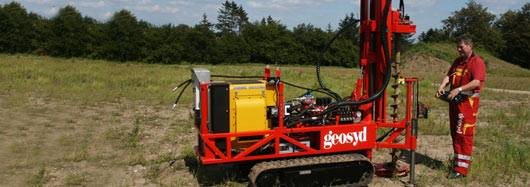
\includegraphics[width=0.50\textwidth]{billeder/Jordbund1}
\caption{Grafik af Aalborgs vækstakse}
\label{fig:Jordbund1}
\end{figure}




Eftersom de fleste øvre jordlag ikke kan holde til vægten af en bygning, bliver man nødt til at finde ud af hvad jorden består af, på en måde som funktion af dybden. Her er der altså tale om de tre jordforhold, Gl, Sg eller Pg. Nogle steder forholder det sig sådan, at jo længere ned man kommer, jo tættere og hårdere vil jorden være. For at fastslå den dybde hvor jorden kan bære og ikke vil sætte sig, er det nødvendigt at foretage jordbundsundersøgelser. 

I vores specifikke tilfælde har vi med en bygning at gøre, som ligger i relativ nærhed af vand. I nærheden af vand varierer jordtyperne meget, og grundvandsspejlets dybde får stor betydning for funderingstypen, samt størrelsen. Foruden dette varierer jordtyperne også meget i nærheden af vand, hvilket fremmer nødvendigheden af en dybdegående jordbundsundersøgelse. Desuden kan der i nærheden af vand skabes opdrift i jorden, da denne er lettere end vandet, hvilket vil skubbe på fundamentet nedefra. Herfor vil det være vanskeligere, uden en jordbundsundersøgelse, at sige med sikkerhed hvor det bærende lerlag befinder sig.


